%!TEX root = ../Dissertation.tex
\section{Problem Formulation}\label{sec:problem}

\blindtext

You might want to try adding some figures. In \ref{fig:an-image}
\begin{figure}\centering
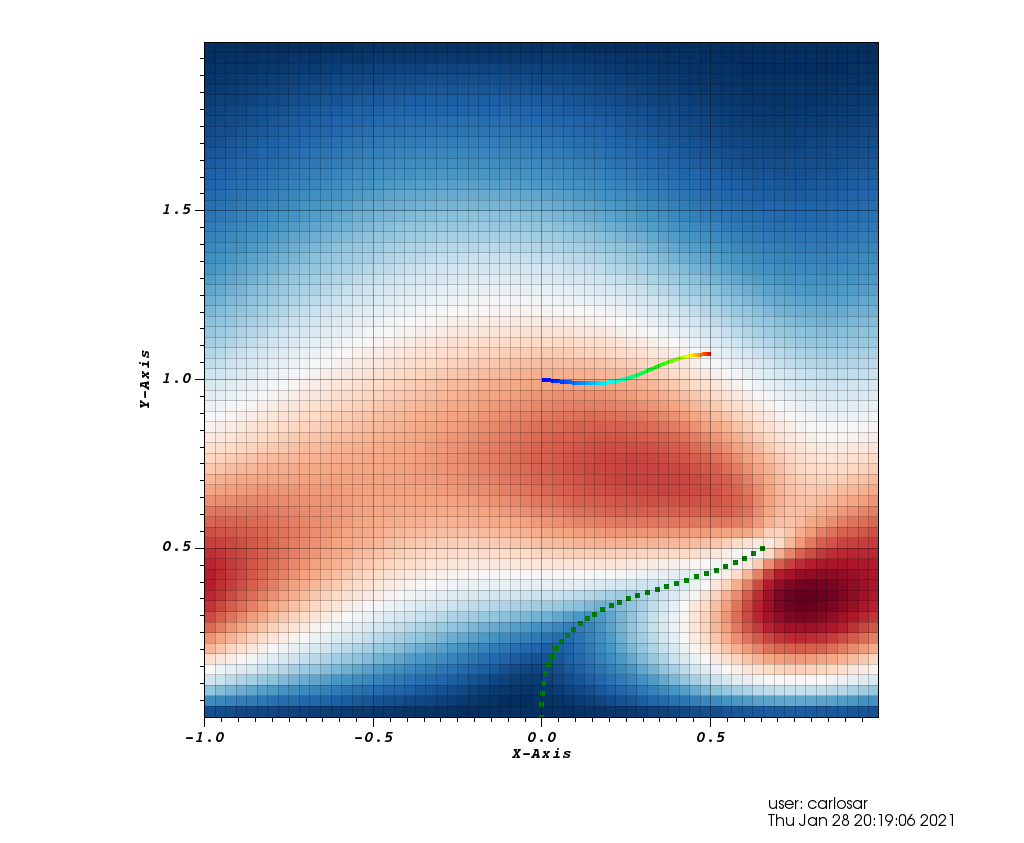
\includegraphics[width=.75\linewidth]{img/cilia-pathline}%
\caption{\label{fig:an-image} Simulation of single cilium.}%
\end{figure}
\blindtext

You also probably need the NS equations. The governing equations of motion for the periciliary fluid are the incompressible Navier-Stokes equations given by Equations \ref{eq:mass_con}-\ref{eq:momentum_con}. 
% conservation of momentum
    \begin{equation} \label{eq:mass_con}
        \vec{\nabla} \cdot \vec{v}(\vec{x},t) = 0
    \end{equation}
    \begin{equation} \label{eq:momentum_con}% conservation of momentum
    % \begin{split}
        \rho_p \left ( \frac{\partial \vec{v}}{\partial t} (\vec{x},t)
        + \vec{\nabla} \cdot (\vec{v}(\vec{x},t) \otimes \vec{v}(\vec{x},t)) \right) 
        = -\vec{\nabla} p (\vec{x},t)
        + \mu_{p}\vec{\nabla}^2 \vec{v} (\vec{x},t)
        + \vec{f}_b(\vec{x},t)
    % \end{split}
    \end{equation}
Equation \ref{eq:mass_con} is the incompressible mass continuity equation, and Equation \ref{eq:momentum_con} is the momentum equation, where the parameters...

\section{More testing of things}
I also used subcaption to get some subfigures (Figure \ref{fig:subfigures}), and changed the caption margin to add some spacing between the figure subcaptions. Figure \ref{fig:subfigure1} and \ref{fig:subfigure2} the caption margin makes it look like one continuous caption between the two figures. Downside is that then you might need to add extra lines with invisible text to line them all up. Figure \ref{fig:subfigure0} is not aligned with all of them.
\begin{figure}
    \centering
    \begin{subfigure}[h!]{0.32\textwidth}\captionsetup{margin=0.25cm}
        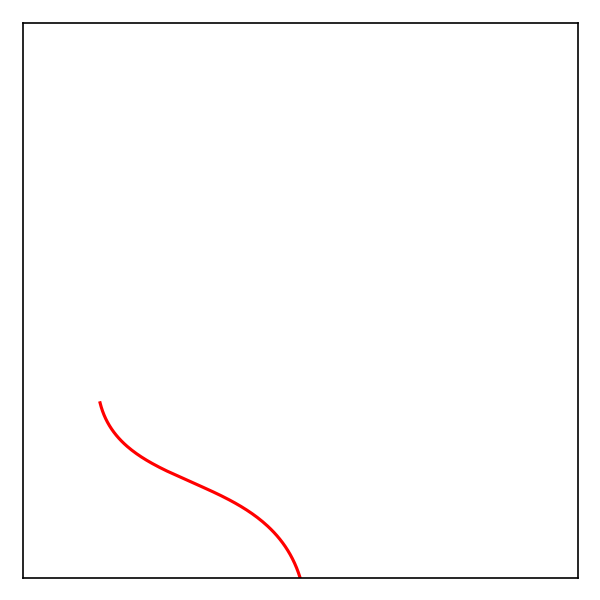
\includegraphics[width=\linewidth]{img/subfolder1/cilia_img0.png}
        \caption{Start of stroke. Long sentence to display the caption margin limits, if it is off, it looks like Figure \ref{fig:subfigure2} and \ref{fig:subfigure1}.}
        \label{fig:subfigure0}
    \end{subfigure}
    \begin{subfigure}[h!]{0.32\textwidth}%\captionsetup{margin=0.25cm}
        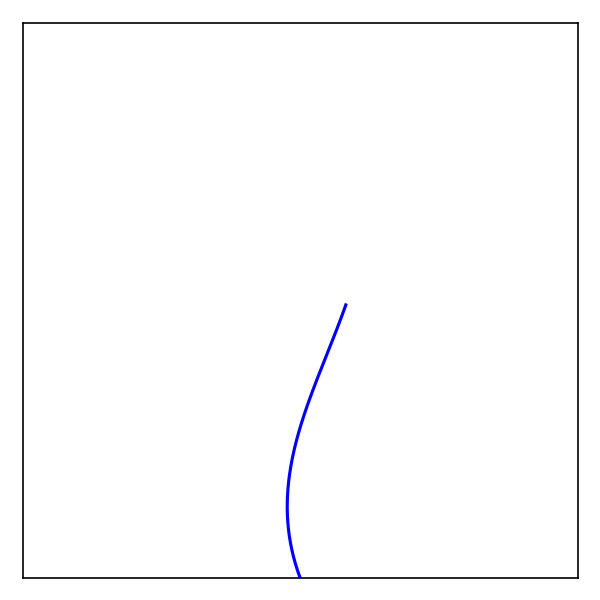
\includegraphics[width=\linewidth]{img/subfolder1/cilia_img1.png}
        \caption{Forward stroke. Long sentence to displace the caption margin limits, if it is off,  it looks like...wait that's us!}
        \label{fig:subfigure1}
    \end{subfigure}
    \begin{subfigure}[h!]{0.32\textwidth}%\captionsetup{margin=0.25cm}
        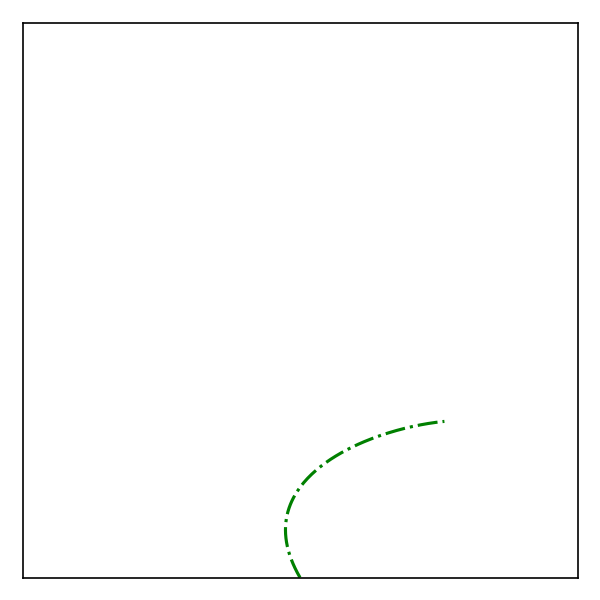
\includegraphics[width=\linewidth]{img/subfolder1/cilia_img2.png}
        \caption{Backward stroke. Long sentence to displace the caption margin limits, if it is off, it looks like...wait that's us!}
        \label{fig:subfigure2}
    \end{subfigure}
    \caption{Some subfigures.}
    \label{fig:subfigures}
\end{figure}

